\documentclass[conference]{IEEEtran}

\usepackage{hyperref}


  
% *** MISC UTILITY PACKAGES ***
%
%\usepackage{ifpdf}
% Heiko Oberdiek's ifpdf.sty is very useful if you need conditional
% compilation based on whether the output is pdf or dvi.
% usage:
% \ifpdf
%   % pdf code
% \else
%   % dvi code
% \fi
% The latest version of ifpdf.sty can be obtained from:
% http://www.ctan.org/tex-archive/macros/latex/contrib/oberdiek/
% Also, note that IEEEtran.cls V1.7 and later provides a builtin
% \ifCLASSINFOpdf conditional that works the same way.
% When switching from latex to pdflatex and vice-versa, the compiler may
% have to be run twice to clear warning/error messages.

% *** GRAPHICS RELATED PACKAGES ***
%
\ifCLASSINFOpdf
  \usepackage[pdftex]{graphicx}
  % declare the path(s) where your graphic files are
  %\graphicspath{{../img/}{../jpeg/}}
  % and their extensions so you won't have to specify these with
  % every instance of \includegraphics
  % \DeclareGraphicsExtensions{.pdf,.jpeg,.png}
\else
  % or other class option (dvipsone, dvipdf, if not using dvips). graphicx
  % will default to the driver specified in the system graphics.cfg if no
  % driver is specified.
  % \usepackage[dvips]{graphicx}
  % declare the path(s) where your graphic files are
  % \graphicspath{{../eps/}}
  % and their extensions so you won't have to specify these with
  % every instance of \includegraphics
  % \DeclareGraphicsExtensions{.eps}
\fi
% graphicx was written by David Carlisle and Sebastian Rahtz. It is
% required if you want graphics, photos, etc. graphicx.sty is already
% installed on most LaTeX systems. The latest version and documentation can
% be obtained at: 
% http://www.ctan.org/tex-archive/macros/latex/required/graphics/
% Another good source of documentation is "Using Imported Graphics in
% LaTeX2e" by Keith Reckdahl which can be found as epslatex.ps or
% epslatex.pdf at: http://www.ctan.org/tex-archive/info/
%
% latex, and pdflatex in dvi mode, support graphics in encapsulated
% postscript (.eps) format. pdflatex in pdf mode supports graphics
% in .pdf, .jpeg, .png and .mps (metapost) formats. Users should ensure
% that all non-photo figures use a vector format (.eps, .pdf, .mps) and
% not a bitmapped formats (.jpeg, .png). IEEE frowns on bitmapped formats
% which can result in "jaggedy"/blurry rendering of lines and letters as
% well as large increases in file sizes.
%
% You can find documentation about the pdfTeX application at:
% http://www.tug.org/applications/pdftex

% *** MATH PACKAGES ***
%
%\usepackage[cmex10]{amsmath}
% A popular package from the American Mathematical Society that provides
% many useful and powerful commands for dealing with mathematics. If using
% it, be sure to load this package with the cmex10 option to ensure that
% only type 1 fonts will utilized at all point sizes. Without this option,
% it is possible that some math symbols, particularly those within
% footnotes, will be rendered in bitmap form which will result in a
% document that can not be IEEE Xplore compliant!
%
% Also, note that the amsmath package sets \interdisplaylinepenalty to 10000
% thus preventing page breaks from occurring within multiline equations. Use:
%\interdisplaylinepenalty=2500
% after loading amsmath to restore such page breaks as IEEEtran.cls normally
% does. amsmath.sty is already installed on most LaTeX systems. The latest
% version and documentation can be obtained at:
% http://www.ctan.org/tex-archive/macros/latex/required/amslatex/math/

% *** SPECIALIZED LIST PACKAGES ***
%
%\usepackage{algorithmic}
% algorithmic.sty was written by Peter Williams and Rogerio Brito.
% This package provides an algorithmic environment fo describing algorithms.
% You can use the algorithmic environment in-text or within a figure
% environment to provide for a floating algorithm. Do NOT use the algorithm
% floating environment provided by algorithm.sty (by the same authors) or
% algorithm2e.sty (by Christophe Fiorio) as IEEE does not use dedicated
% algorithm float types and packages that provide these will not provide
% correct IEEE style captions. The latest version and documentation of
% algorithmic.sty can be obtained at:
% http://www.ctan.org/tex-archive/macros/latex/contrib/algorithms/
% There is also a support site at:
% http://algorithms.berlios.de/index.html
% Also of interest may be the (relatively newer and more customizable)
% algorithmicx.sty package by Szasz Janos:
% http://www.ctan.org/tex-archive/macros/latex/contrib/algorithmicx/

% *** ALIGNMENT PACKAGES ***
%
%\usepackage{array}
% Frank Mittelbach's and David Carlisle's array.sty patches and improves
% the standard LaTeX2e array and tabular environments to provide better
% appearance and additional user controls. As the default LaTeX2e table
% generation code is lacking to the point of almost being broken with
% respect to the quality of the end results, all users are strongly
% advised to use an enhanced (at the very least that provided by array.sty)
% set of table tools. array.sty is already installed on most systems. The
% latest version and documentation can be obtained at:
% http://www.ctan.org/tex-archive/macros/latex/required/tools/

%\usepackage{mdwmath}
%\usepackage{mdwtab}
% Also highly recommended is Mark Wooding's extremely powerful MDW tools,
% especially mdwmath.sty and mdwtab.sty which are used to format equations
% and tables, respectively. The MDWtools set is already installed on most
% LaTeX systems. The lastest version and documentation is available at:
% http://www.ctan.org/tex-archive/macros/latex/contrib/mdwtools/

% IEEEtran contains the IEEEeqnarray family of commands that can be used to
% generate multiline equations as well as matrices, tables, etc., of high
% quality.

%\usepackage{eqparbox}
% Also of notable interest is Scott Pakin's eqparbox package for creating
% (automatically sized) equal width boxes - aka "natural width parboxes".
% Available at:
% http://www.ctan.org/tex-archive/macros/latex/contrib/eqparbox/

% *** SUBFIGURE PACKAGE ***
% subfig.sty, also written by Steven Douglas Cochran, is the modern
% replacement for subfigure.sty. However, subfig.sty requires and
% automatically loads Axel Sommerfeldt's caption.sty which will override
% IEEEtran.cls handling of captions and this will result in nonIEEE style
% figure/table captions. To prevent this problem, be sure and preload
% caption.sty with its "caption=false" package option. This is will preserve
% IEEEtran.cls handing of captions. Version 1.3 (2005/06/28) and later 
% (recommended due to many improvements over 1.2) of subfig.sty supports
% the caption=false option directly:
\usepackage[caption=false,font=footnotesize]{subfig}
      
%
% The latest version and documentation can be obtained at:
% http://www.ctan.org/tex-archive/macros/latex/contrib/subfig/
% The latest version and documentation of caption.sty can be obtained at:
% http://www.ctan.org/tex-archive/macros/latex/contrib/caption/

% *** FLOAT PACKAGES ***
%
%\usepackage{fixltx2e}
% fixltx2e, the successor to the earlier fix2col.sty, was written by
% Frank Mittelbach and David Carlisle. This package corrects a few problems
% in the LaTeX2e kernel, the most notable of which is that in current
% LaTeX2e releases, the ordering of single and double column floats is not
% guaranteed to be preserved. Thus, an unpatched LaTeX2e can allow a
% single column figure to be placed prior to an earlier double column
% figure. The latest version and documentation can be found at:
% http://www.ctan.org/tex-archive/macros/latex/base/

%\usepackage{stfloats}
% stfloats.sty was written by Sigitas Tolusis. This package gives LaTeX2e
% the ability to do double column floats at the bottom of the page as well
% as the top. (e.g., "\begin{figure*}[!b]" is not normally possible in
% LaTeX2e). It also provides a command:
%\fnbelowfloat
% to enable the placement of footnotes below bottom floats (the standard
% LaTeX2e kernel puts them above bottom floats). This is an invasive package
% which rewrites many portions of the LaTeX2e float routines. It may not work
% with other packages that modify the LaTeX2e float routines. The latest
% version and documentation can be obtained at:
% http://www.ctan.org/tex-archive/macros/latex/contrib/sttools/
% Documentation is contained in the stfloats.sty comments as well as in the
% presfull.pdf file. Do not use the stfloats baselinefloat ability as IEEE
% does not allow \baselineskip to stretch. Authors submitting work to the
% IEEE should note that IEEE rarely uses double column equations and
% that authors should try to avoid such use. Do not be tempted to use the
% cuted.sty or midfloat.sty packages (also by Sigitas Tolusis) as IEEE does
% not format its papers in such ways.

% correct bad hyphenation here
\hyphenation{}

%\usepackage{multicol}
%\usepackage{multirow}
\usepackage{ntheorem}
\usepackage{hyperref}

%\usepackage{fancyvrb}
%\usepackage{longtable, lscape}
%\usepackage{setspace}
%\usepackage{float}

\usepackage{framed}
\usepackage[listings,skins]{tcolorbox}
\usepackage[skipbelow=\topskip,skipabove=\topskip]{mdframed}

% Umkreiste Zahlen
\usepackage{tikz}
\usetikzlibrary{trees,arrows,positioning, calc, shapes.geometric} 

% Node Styles
\tikzstyle{root}=[draw,fill=gray,rectangle,minimum size=8pt,inner sep=0pt,label={0:root}]
\tikzstyle{read}=[draw,fill=blue,circle,minimum size=8pt,inner sep=0pt,label={0:read}]
\tikzstyle{mod}=[draw,fill=magenta,circle,minimum size=8pt,inner sep=0pt,label={0:mod}]
\tikzstyle{memo}=[draw,fill=green!50,shape=diamond,minimum size=8pt,inner sep=0pt,label={0:memo}]
\tikzstyle{write}=[draw,fill=orange,circle,minimum size=8pt,inner sep=0pt,label={0:write}]
\tikzstyle{par}=[draw,fill=yellow,shape=diamond,minimum size=8pt,inner sep=0pt,label={0:par}]

% Definition
\usepackage{amsmath} 
%\theoremstyle{definition}
   \newtheorem{definition}{Definition}
   \newtheorem{definition-non}{Definition}
%\theoremstyle{plain}
    \newtheorem{theorem}{Theorem}
    \newtheorem{theorem-non}{Theorem}  
    \newtheorem{lemma}{Lemma}
% Mathematische Symbole
\usepackage{amssymb}


\begin{document}

\title{A Practical Approach to Analyzing Incremental Programs Using Execution Traces}

\author{\IEEEauthorblockN{Walter Tichy, Umut Acar, Thomas Marshall, Emanuel J\"{o}bstl}
\IEEEauthorblockA{Karlsruhe Institute of Technology, Faculty of Computer Science\\
Carnegie Mellon University, Computer Science Department\\
}}

\maketitle

\begin{abstract}
The principle of incremental programming has been well known for many years. While the automatic transformation of sequential programs into efficient incremental programs is not solved in general, a number of platforms for incremental computation have been created. In this document, we inspect the incremental computation platform TBD. First, we summarize known principles like directed dependency graphs, execution traces, intrinsic trace distance and trace stability, then we create an program model which enables us to apply those principles to TBD programs. We also present an algorithm to calculate the intrinsic trace distance in practice. Finally, we show how we can make automatic optimizations to programs by analyzing the dependency graph. 
\end{abstract}

%\begin{IEEEkeywords}
%Incremental computing, tbd, scala
%\end{IEEEkeywords}

\IEEEpeerreviewmaketitle
%
% -----------------------------
%

\section{Introduction}
This section should describe the purpose of incremental computation and also explain for which purpose the concept of incremental computation is useful. 

\subsection{Approaches to incremental computation}
This subsection should describe various historic approaches to incremental computation. This includes, but is not limited to: 

\subsection{Naiad and TBD}
This subsection should shortly outline Naiad and TBD. Additionally, the choice of comparing Naiad to TBD should be explained. 

\section{Fundamental work}
The work of U. Acar et al\cite{Acar2005thesis} describes the theoretical and practical concept of incremental computing using memorization and DDGs in detail. Since these concepts are important for understanding this writing, they are summarized in this section. First, general terms are explained briefly, then, a short theoretical outline for the term of stable algorithms is provided. 

\subsection{Change Propagation, Dynamic Dependence Graphs and Memorization}

A \textit{Dynamic Dependence Graph (DDG)} can be described as a data structure, which holds a directed graph for tracking control and data dependencies during execution \cite{Acar2005thesis}, whereas the nodes of the graph are usually function calls in the program. In contrast to \textit{Static Dependence Graphs} \cite{Demers1981}, DDGs are mutated during change propagation and therefore adjusted to the new program structure. 

\textit{Memorization} is the concept of storing intermediate results and re-using them during change propagation. Memorization can be combined with DDGs, by inserting memorization nodes into the graph. During change propagation, this can lead to a significant performance increase, because entire sub-trees of the call graph and their corresponding results can be re-used \cite{Acar2005thesis}. 

\subsection{Execution Traces}

\label{sec:ddg_memo}
A trace is a theoretical construct which can be described as an ordered tree, whereas nodes represent function calls during the program execution \cite{Acar2005thesis}. While similar to the DDG, a trace tracks no data dependencies. A trace usually resembles the call tree of a program. 

\begin{definition}[General trace node equality]
Each node $v$ is uniquely described by a tag, consisting of

\begin{itemize}
\item the function being called, $fun(v)$
\item the arguments of the function call, $args(v)$
\item the values read in the body of the function, $reads(v)$
\item the values returned to the function from its callees, $returns(v)$
\item the weight of the function, $w(v)$, which is equal to its execution time.
\end{itemize}

Two nodes $v$ and $v'$ are equal, denoted $v \equiv v'$, if $fun(v) = fun(v')$, $args(v) = args(v')$, $reads(v) = reads(v')$ and $returns(v) = returns(v')$.
\end{definition}

\subsection{Trace distance}
Trace distance can basically be described as an edit distance between two execution traces \cite{Acar2005thesis} \cite{acar2004dynamizing}. 

To find the minimum trace distance of two traces $T$ and $T'$, the so called \textit{cognates} relation can be used. 

\begin{definition}[Cognates]
A set of cognates $C$ is a relation of two traces $T$ and $T'$ with the set of nodes $V$ and $V'$, so that

\begin{itemize}
\item $C \subset V \times V'$
\item for each $(v, v') \in V: v \equiv v'$ 
\item no node is paired with more than one node
\end{itemize}
\end{definition}
All nodes of both traces $T$ and $T'$ can be colored either blue, yellow or red. 
Nodes which have a cognate are colored blue. Nodes of $T$ without a cognate are colored yellow. Nodes of $T'$ without a cognate are colored red. 

The trace distance can now be calculated by summing up the weights of all yellow and red nodes. 

\begin{definition}[Trace distance]
The trace distance $\delta(T, T')$ between two traces $T$ and $T'$ is given by
\begin{align*}
	\delta(T, T') = \sum_{y \in Y} w(y) + \sum_{r \in R} w(r)
\end{align*}
whereas $Y$ denotes the set of all yellow vertices and $R$ is the set of all red vertices. 
\end{definition}

If the cognate relation $C$ is maximal, the intrinsic distance is minimal, denoted as $\delta^{min}$. Also, a maximal cognate relation can be found using a naive greedy algorithm \cite{Acar2005thesis} \cite{acar2004dynamizing}.

The minimal trace distance forms a lower bound for the duration of change propagation, since during change propagation all red vertices have to be deleted, and all yellow vertices have to be re-evaluated \cite{Acar2005thesis}. 

\subsection{Stability of algorithms}

When we inspect change propagation not only for a single run, but for all possible runs of an algorithm, we can find an upper bound for the expected time of change propagation. This upper bound, denoted in Landau notation as $O(f(n))$, expresses the expected time for change propagation for a change of a constant number of elements in the input data \cite{Acar2005thesis}. 

If the expected time for change propagation of an algorithm $A$ lies within $O(f(n))$, the algorithm is called $O(f(n))$\textit{-stable}. 
Algorithms which are $O(g(n))$-stable are called \textit{stable algorithms} \cite{Acar2005thesis}, if $g(n)$ is a sub-linear growing function.
\section{TBD}
\label{sec:tbd}
The \textit{TBD} (\textit{T}o\textit{B}e\textit{D}etermined) platform is a framework for incremental computation currently being developed at Carnegie Mellon University (CMU). TBD follows the approach of memorization combined with directed dependency graphs (DDGs), as throughly described in \cite{Acar2005thesis}. Also, parallel computing is supported. The framework allows a programmer to write software using TBDs programming interface, while TBD automatically takes care about invoking the correct functions for change propagation, in case of an update of the input data.
The framework is being developed in the Scala language, which enables us to exploit the reflection capabilities of Scala for analysis \cite{burmako2013scala} \cite{stocker2010scala}. 
The source code of TBD is available at \hyperref[]{https://github.com/twmarshall/tbd}. 

\subsection{Programming interface} 
TBD needs to keep track of reads and writes of variables in the program. To accomplish this, TBD wraps all values relevant for change propagation into so called \textit{modifiables} or short \textit{Mods}. TBD automatically wraps all input data into Mods. 

\subsubsection{mod}
To create Mods, for example as result of the program execution, TBD provides a method $mod$. The declaration of $mod$ can be seen in listing \ref{code:mod}. The $mod$ method calls a function parameter $initializer$ with a \textit{destination} or \textit{Dest} as argument. The value written to the Dest by the function parameter is then stored in the Mod, which is returned by the $mod$ method. Requiring the return type of \textit{Changeable} simply enforces that a write is the last operation inside $initializer$. 

\begin{figure}
\begin{lstlisting}[frame=single,basicstyle=\ttfamily]
def mod[T](
  initializer: Dest[T] => Changeable[T]
): Mod[T]
\end{lstlisting}
\caption{Signature of the $mod$ method}
\label{code:mod}
\end{figure}

\subsubsection{write}
To write to a Dest, TBD provides a $write$ method. The signature of $write$ can be found in listing \ref{code:write}. The $write$ method simply takes a Dest and a value, and writes the value to the given Dest. The write method returns a Changeable. 

\begin{figure}
\begin{lstlisting}[frame=single,basicstyle=\ttfamily]
def write[T](
    dest: Dest[T], 
    value: T
): Changeable[T]
\end{lstlisting}
\caption{Signature of the $write$ method}
\label{code:write}
\end{figure}

\subsubsection{read}
The values from within modifiables have to be read explicitly. For this purpose, TBD provides a $read$ method, which accepts a Mod as parameter and then calls a function parameter $reader$ with the value of the Mod as first argument. The signature can be seen in in listing \ref{code:read}. For $read$, the function parameter $reader$ also has to return a Changeable. Reads without an enclosed write are not useful, since the $read$ method my not modify values outside of it's scope.  

\begin{figure}
\begin{lstlisting}[frame=single,basicstyle=\ttfamily]
def read[T, U <: Changeable[_]](
    mod: Mod[T], 
    reader: T => U
): U
\end{lstlisting}
\caption{Signature of the $read$ method}
\label{code:read}
\end{figure}

Listing \ref{code:simpleExample} shows a very simple example, which adds two Mods of type integer. First, $mod$ is called to create a Dest for the result, then the values of $mod1$ and $mod2$ are read. The values of $mod1$ and $mod2$ are then added and written to $dest$. The nesting of functions as seen in the example is typical for applications on top of TBD. 

\begin{figure}
\begin{lstlisting}[frame=single,basicstyle=\ttfamily]
def add(
    tbd: TBD, 
    mod1: Mod[Int], 
    mod2: Mod[Int]
): Mod[Int]) = {
    tbd.mod((dest: Dest[Int]) => {
        tbd.read(mod1)(v1 => {
            tbd.read(mod2)(v2 => {
                tbd.write(dest, v1 + v2)
            })
        })
    })
}
\end{lstlisting}
\caption{A basic example, utilizing $read$, $write$, and $mod$}
\label{code:simpleExample}
\end{figure}

Since all programs consist of $read$, $write$ and $mod$ functions, and all Modifiables have to be explicitly written, TBD is able to construct a DDG from monitoring the calls to the corresponding functions.

\subsubsection{memo}
As we already mentioned, TBD not only utilizes DDGs, but also memorization. To accomplish memorization, TBD provides a method to create so-called \textit{Lifts}, which in turn provide a method for memorization, $memo$. The $memo$ method accepts a list of parameters, which are used to match this $memo$ call and a function parameter $func$. A Lift can be described as memorization context. Calling $memo$ with the same parameters as any previous call on the same Lift will yield the same result, without evaluation $func$. If there is no match, $func$ will be called and the result will be stored for future memorization. In general, it is important to not share Lift objects between unrelated function calls, but to preserve the same Lift for all calls to the same function. The signature of $memo$ can be seen in listing \ref{code:memo}.

\begin{figure}
\begin{lstlisting}[frame=single,basicstyle=\ttfamily]
def memo(
    args: List[_], 
    func: () => T
): T
\end{lstlisting}
\caption{Signature of the $memo$ method}
\label{code:memo}
\end{figure}

A typical use case for memorization is list processing. A typical example is shown in \ref{code:memoExample}. First, we define a class for list nodes and the properties $value$ of type integer and $next$. Note that the class is immutable. Next, we define a function, $incrementalList$, which initializes a lift and calls a recursive function, $incrementRecursive$ with the head of the list and the created lift. The latter function maps each list node to a list node with $value$ increased by one. This is done by first creating a Dest $dest$ for the new List Node. Then, the current node is read from it's modifiable. If the current node is null, the end of the list is reached and $null$ can be written to $dest$. If the current node is not $null$, the value is read, increased, and written again to create the Mod $newValue$, similar to the example in listing \ref{code:simpleExample}. 

Then, $incrementRecursive$ is called recursively with the next node as parameter. The call to $incrementRecursive$, however, is enclosed in a memo operation, with the next node as parameter. If a change propagation happens now, TBD is not going to recursively call all reads again, but will stop as soon as a memo match occurs. This is typically the case as soon as the recursion reaches an unchanged list element. 

In the end, a new list node is constructed from the results and returned. 
\begin{figure*}
\begin{lstlisting}[frame=single,basicstyle=\ttfamily]
class ListNode(_value: Mod[Int], _next: Mod[ListNode]) {
    val value = _value
    val next = _next
}

def incrementList(tbd: TBD, head: Mod[ListNode]): Mod[ListNode] = {
    val lift = tbd.makeLift()
    incrementRecursive(tbd, head, lift)
}

def incrementRecursive(tbd: TBD, current: Mod[ListNode], lift: Lift[ListNode])
    : Mod[ListNode] = {

    tbd.mod((dest: Dest[ListNode]) => {
        tbd.read(current)(current => {
            if(current == null) {
                tbd.write(dest, null)
            } else {
                val newValue = tbd.mod((destValue: Dest[Int]) => {
                    tbd.read(current.value)(value => {
                      tbd.write(destValue, value + 1)
                    })
                })

                val newNext = lift.memo(List(current.next), () => {
                    incrementRecursive(tbd, current.next, lift)
                })

                tbd.write(dest, new ListNode(newValue, newNext))
            } 
        })
    })
}

\end{lstlisting}
\caption{A basic example, utilizing $memo$}
\label{code:memoExample}
\end{figure*}

\subsubsection{par}
The last crucial method offered by TBD is a method to execute code in parallel, $par$. The $par$ method takes two function parameters $one$ and $two$, where each function parameter is executed on a separate worker thread with separate TBD objects. The $par$ method blocks until both workers are finished. The signature of $par$ is shown in listing \ref{code:par}

\begin{figure}
\begin{lstlisting}[frame=single,basicstyle=\ttfamily]
def par[T, U](
    one: TBD => T, 
    two: TBD => U
): Tuple2[T, U] 
\end{lstlisting}
\caption{Signature of the $par$ method}
\label{code:par}
\end{figure}

\subsection{Constraints and responsibilities}
\label{sec:constraints}
During change propagation, TBD re-evaluates all $read$ calls that read modifiables which have changed, in the same order they were called during the initial run. Obviously, the functions invoked $read$, $mod$, $memo$ and $par$ may not write variables outside of their scope, or they will easily break change propagation. They have to be side effect free. 

If, for example, a static variable is written from within a function called by read, and then used somewhere else in the program, the system has no way to propagate a change of this variable.

Furthermore, all functions called have to be deterministic. Calling the same function with the same parameters has to lead to the same return value or the same value written to a dest. Otherwise, memorization will not be usable in the program.

For each function parameter passed to the functions $read$ or $mod$, the last operation executed in that function parameter has to be a $write$. This is enforced by requiring the return type of $Changeable$ for function parameters.
Due to this, it is generally not possible to use return statements to return values within a TBD program.  
\section{Theoretic fundamentals}
While a very comprehensive theoretical model for incremental programs based on DDGs and memorization can be found in \cite{Acar2005thesis}, we have to adjust parts of the model to fit the TBD platform. The concept of a \textit{trace} is necessary as a fundamental approach for gathering information about an incremental program. The approach of \textit{trace distance} is important for the analysis of programs, since it can be used as a metric for the performance of the change propagation of a given incremental algorithm. 

\subsection{Execution Traces}

\label{sec:ddg_memo}
A trace is a theoretical construct which can be described as an ordered tree, whereas nodes represent function calls during the program execution \cite{Acar2005thesis}. While similar to the DDG, a trace tracks no data dependencies. A trace usually resembles the call tree of a program. 

\begin{definition}[General trace node equality]
Each node $v$ is uniquely described by a tag, consisting of

\begin{itemize}
\item the function being called, $fun(v)$
\item the arguments of the function call, $args(v)$
\item the values read in the body of the function, $reads(v)$
\item the values returned to the function from its callees, $returns(v)$
\item the weight of the function, $w(v)$, which is equal to its execution time.
\end{itemize}

Two nodes $v$ and $v'$ are equal, denoted $v \equiv v'$, if $fun(v) = fun(v')$, $args(v) = args(v')$, $reads(v) = reads(v')$ and $returns(v) = returns(v')$.
\end{definition}

\subsection{Trace distance}
Trace distance can basically be described as an edit distance between two execution traces \cite{Acar2005thesis} \cite{acar2004dynamizing}. 

To find the minimum trace distance of two traces $T$ and $T'$, the so called \textit{cognates} relation can be used. 

\begin{definition}[Cognates]
A set of cognates $C$ is a relation of two traces $T$ and $T'$ with the set of nodes $V$ and $V'$, so that

\begin{itemize}
\item $C \subset V \times V'$
\item for each $(v, v') \in V: v \equiv v'$ 
\item no node is paired with more than one node
\end{itemize}
\end{definition}
All nodes of both traces $T$ and $T'$ can be colored either blue, yellow or red. 
Nodes which have a cognate are colored blue. Nodes of $T$ without a cognate are colored yellow. Nodes of $T'$ without a cognate are colored red. 

The trace distance can now be calculated by summing up the weights of all yellow and red nodes. 

\begin{definition}[Trace distance]
The trace distance $\delta(T, T')$ between two traces $T$ and $T'$ is given by
\begin{align*}
  \delta(T, T') = \sum_{y \in Y} w(y) + \sum_{r \in R} w(r)
\end{align*}
whereas $Y$ denotes the set of all yellow vertices and $R$ is the set of all red vertices. 
\end{definition}

If the cognate relation $C$ is maximal, the intrinsic distance is minimal, denoted as $\delta^{min}$. Also, a maximal cognate relation can be found using a naive greedy algorithm \cite{Acar2005thesis} \cite{acar2004dynamizing}.

The minimal trace distance forms a lower bound for the duration of change propagation, since during change propagation all red vertices have to be deleted, and all yellow vertices have to be re-evaluated \cite{Acar2005thesis}.

\subsection{Traces in TBD}

While we can retain the definition of a trace, we have to adjust the definition of nodes and node equality for our purpose, so we can use it in the next section to construct an algorithm for trace distance calculation usable on the TBD platform. 

\subsubsection{TBD trace nodes}
As described in section \ref{sec:tbd}, TBD provides $read$, $mod$, $write$, $memo$ and $par$ methods to the developer. Instead of creating an execution trace out of all  functions in the program, we restrict ourselves to a trace consisting of only these functions. It should be noted, that, since we require each function to be side-effect free and deterministic, we could theoretically omit $write$ nodes in the DDG, since they directly depend on their corresponding parent nodes. However, including these nodes can provide useful insights during debugging. 

\begin{definition}[TBD Trace nodes]
Let each node in our execution trace represent a $read$, $mod$, $write$ $memo$ or $par$ function. We annotate each node with a tuple of the following values:
\begin{itemize}
\item the node type $t$, which can have the values $read$, $mod$, $write$, $memo$ or $par$
\item a node tag, a sequence of labels which has a different structure depending on the node type 
\end{itemize}
\end{definition}

Depending on the node type, we define the following node tags: 

\begin{definition}
Let the tag for $read$ nodes consist of $\mathbf{(a, fun)}$, whereas
\begin{itemize}
\item $a$ is the value of the modifiable being read
\item $fun$ is the reader function being called
\end{itemize}
\end{definition}

\begin{definition}
Let the tag for $mod$ nodes consist of $\mathbf{(fun)}$, whereas
\begin{itemize}
\item $d$ is the id of the destination generated by this call
\item $fun$ is the initializer function being called
\end{itemize}
\end{definition}

\begin{definition}
Let the tag for $write$ nodes consist of $\mathbf{(a, d)}$, whereas
\begin{itemize}
\item $a$ is the value being written
\item $d$ is the id of the destination where $a$ is being written to 
\end{itemize}
\end{definition}

\begin{definition}
Let the tag for $memo$ nodes consist of $\mathbf{((a_1, ..., a_n), fun)}$, whereas
\begin{itemize}
\item $(a_1, ..., a_n)$ is the list of values to memo match against
\item $fun$ is the function being called
\end{itemize}
\end{definition}

\begin{definition}
Let the tag for $par$ nodes consist of $\mathbf{(fun_1, fun_2)}$, whereas
\begin{itemize}
\item $fun_1$ is the first function being called
\item $fun_2$ is the second function being called
\end{itemize}
\end{definition}

\subsubsection{TBD trace node equality}
\label{sec:node_equality}
Given these definitions, we now re-define equality of nodes. 

\begin{definition}[Node equality]
Let a node $A$ and $B$ be equal, iff the node type of $A$, $t_a$, equals the node type of $B$, $t_b$, and the tag of $A$ equals the tag of $B$. 
\end{definition}
We only compare the the tag if the node type already matches. Therefore, we can simply compare each element in the tag of $A$ with it's counterpart in the tag of $B$. 

The tag can consist of objects, value types, modifiables or functions. For functions, showing equality is not solvable in general \cite{church1936note}. With the constraints of TBD programs, however, we are able to create a sufficient equality definition for our purpose.
\begin{definition}[Function execution equality for TBD traces]
\label{def:fun_equality}
A function execution $fun_a$ and a function execution $fun_b$ are equal, iff all of the following conditions apply: 
\begin{enumerate}
\item $fun_a$ and $fun_b$ refer to the same symbol in the source code. 
\item all arguments are equal.
\item all free variables bound from an outer scope are equal. 
\end{enumerate}
\end{definition}

The requirement for side-effect free and deterministic functions leads to the conclusion, that all sub calls to other functions, including any writes, are going to be equal if the function is invoked with the same parameters. We have to take care of free variables in the function, however, since they might influence the behavior of the program. An example would be a $read$ nested within another $read$, whereas the inner $read$ accesses the value provided by the outer read, which can be seen in listing \ref{code:simpleExample}. If the value of $mod1$ changes in the example the inner function performing the addition of $v1$ and $v2$ is not going to be equal anymore, therefore the $read$ node of the inner $read$ has changed, even the value of $mod2$ stays the same. 

For comparing values or objects inside the tag, function parameters or closed free variables we use \textit{deep equality}. Modifiables, however should be compared by reference equality. The reason for doing so is to ensure correctness even with complex types, for example like arrays, nested lists or objects. For modifiables, the change propagation algorithm takes care of changed values, and automatically calls all sub calls which are affected. The case where the modifiable itself was re-created forms an exception, where we would have to re-execute all reads which would access this modifiable. This leads to the following formal definition: 

\begin{definition}[Object equality for TBD traces]
A primitive value $p$ is equal to a primitive value $k$ iff $p$ and $k$ have the same type and the same value. 

A modifiable $x$ is equal to a modifiable $y$ iff $x$ and $y$ refer to the same object in memory.

An object $A$ with ordered properties $(a_1, ..., a_n)$ is equal to an object $B$ with ordered properties  $(b_1, ..., b_n)$ iff $A$ and $B$ have the same type and $a_i$ equals $b_i$ $\forall i \in[1, n]$. Properties of an object can be other objects, modifiables or primitives. 
\end{definition}

With these definition of trace node equality, we can keep the definition of $Cognates$ and $Trace Distance$ given in in section \ref{sec:ddg_memo}.

Figure \ref{tree:incrementListTrace} illustrates a trace of a TBD program. The program executed here is the example found in listing \ref{code:memoExample}. The input consists of a list of three elements, 1, 2 and 3 in this case. Values of the form $d.\alpha$ inside the tag denote dests or mods, whereas $\alpha$ is the unique key. Values of the form $f.\delta $ inside the tag denote anonymous functions, whereas $\delta $ is an automatically generated unique identifier. 

\begin{figure}
\centering
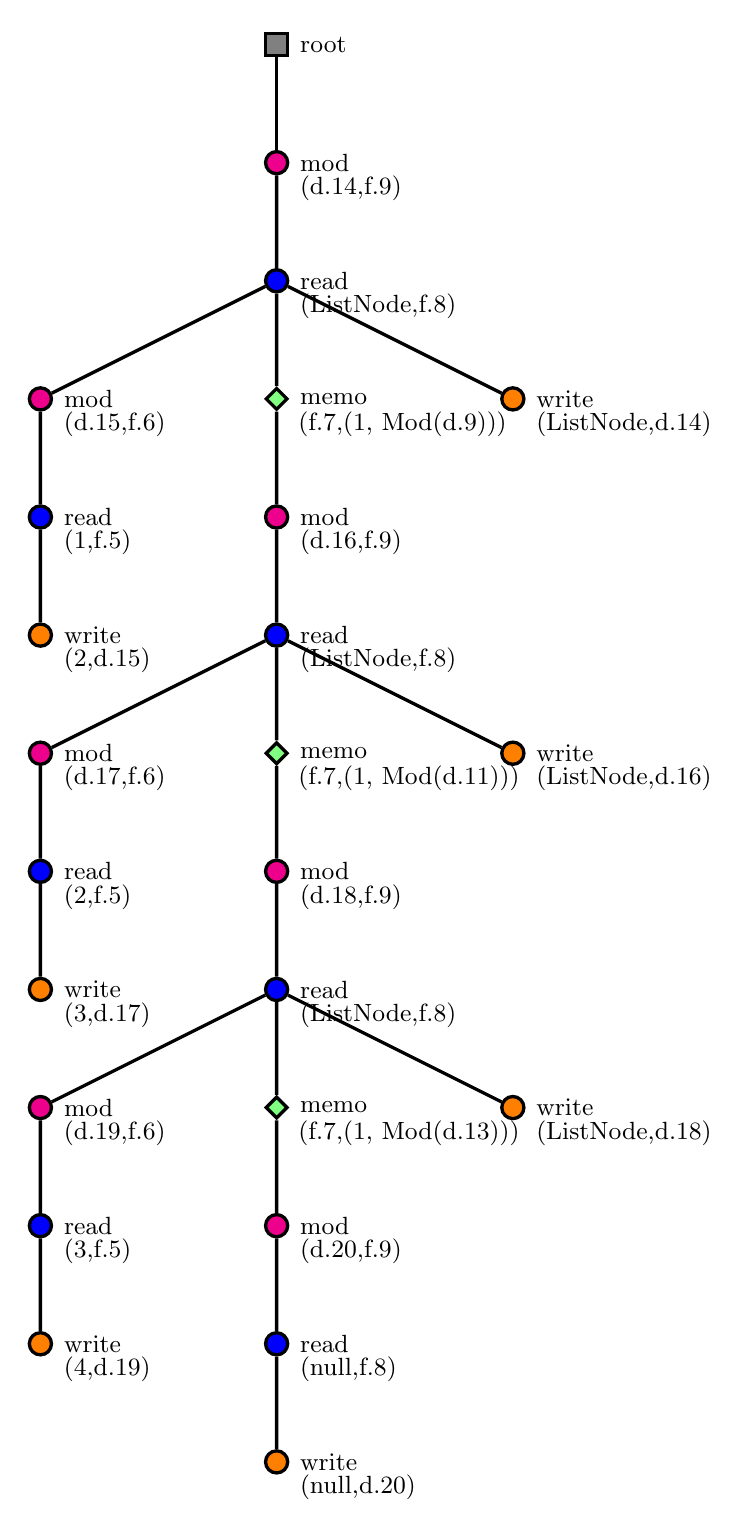
\begin{tikzpicture}[font=\sffamily,very thick,level/.style={sibling distance=30mm}]
\tikzstyle{every node}=[font=\small]
\node [root]{}
child {
  node [mod, label={350:(d.14,f.9)}]{}
  child {
    node [read, label={350:(ListNode,f.8)}]{}
    child {
      node [mod, label={350:(d.15,f.6)}]{}
      child {
        node [read, label={350:(1,f.5)}]{}
        child {
          node [write, label={350:(2,d.15)}]{}
        }
      }
    }
    child {
      node [memo, label={350:(f.7,(1, Mod(d.9)))}]{}
      child {
        node [mod, label={350:(d.16,f.9)}]{}
        child {
          node [read, label={350:(ListNode,f.8)}]{}
          child {
            node [mod, label={350:(d.17,f.6)}]{}
            child {
              node [read, label={350:(2,f.5)}]{}
              child {
                node [write, label={350:(3,d.17)}]{}
              }
            }
          }
          child {
            node [memo, label={350:(f.7,(1, Mod(d.11)))}]{}
            child {
              node [mod, label={350:(d.18,f.9)}]{}
              child {
                node [read, label={350:(ListNode,f.8)}]{}
                child {
                  node [mod, label={350:(d.19,f.6)}]{}
                  child {
                    node [read, label={350:(3,f.5)}]{}
                    child {
                      node [write, label={350:(4,d.19)}]{}
                    }
                  }
                }
                child {
                  node [memo, label={350:(f.7,(1, Mod(d.13)))}]{}
                  child {
                    node [mod, label={350:(d.20,f.9)}]{}
                    child {
                      node [read, label={350:(null,f.8)}]{}
                      child {
                        node [write, label={350:(null,d.20)}]{}
                      }
                    }
                  }
                }
                child {
                  node [write, label={350:(ListNode,d.18)}]{}
                }
              }
            }
          }
          child {
            node [write, label={350:(ListNode,d.16)}]{}
          }
        }
      }
    }
    child {
      node [write, label={350:(ListNode,d.14)}]{}
    }
  }
};
\end{tikzpicture}
\caption{Trace of a TBD program [Todo: Find more elegant solution for tags.]}
\label{tree:incrementListTrace}
\end{figure}

The leftmost subtrees correspond to creating a modifiable for the resulting value, reading the input value and writing the result. The central path holds all calls which recursively read the input and handle memorization. The rightmost and bottom $write$ calls write the resulting new list nodes.  

The edges in the trace illustrate control dependencies. However, by observing the keys of dests in the $mod$ and $write$ operations, data dependencies can be found. 

\section{An intrinsic trace distance algorithm for TBD}
While \cite{Acar2005thesis} already outlines a greedy algorithm for calculating the intrinsic trace distance, there are details we have to take care of for accomplishing an implementation.

\subsection{Implementing node equality}
While equality of nodes is defined in section \ref{sec:node_equality}, it still remains open how a equality is implemented. For value types or objects we can use the $equals$ method provided by the Scala platform or define our own overload of $equals$, if needed.  

For testing anonymous functions passed to $read$, $memo$, $mod$, and $par$ for equality, we have to compare the the function itself, all parameters, all arguments, and all free variables bound from an outer scope, as described in definition \ref{def:fun_equality}. To accomplish this task, we can utilize the Scala macro API \cite{burmako2013scala}. Basically, the Scala macro API enables us to define small programs written in Scala, which are executed during compile time. From within these macros, we can access all information the compiler has and modify the abstract syntax tree (AST) of our program on the fly. 

To gather the necessary information for comparing anonymous functions during runtime, we replace the implementations of $read$, $memo$, $mod$ and $par$ with macros, which extract interesting information and create a tag from it. The macro generates code which calls the original function and passes the original parameters and the tag as arguments. 

During macro expansion, we can simply assign an unique ID to each function. This way, we can easily check whether to function tags refer to the same function. The arguments of the function are also well known for all methods provided by TBD, so they can be easily added to the tag. 

Finding free variables which are bound from an outer scope, however, is not straight-forward, because at the macro expansion step, the Scala compiler has no knowledge about whether a symbol is a function or a variable, or from where it is bound.

To extract only the correct symbols, we first create a list of all symbols which occur in the anonymous function $F$ and store them in a set $V = (v_1, ..., v_n)$. Then, for each $v_i$, $i \in[1..n]$, we iterate over all ancestors of $v_i$ in the AST of $F$. If we find a variable definition or parameter which defines a symbol with the same name as $v_i$, we know that $v_i$ is not bound from an outer scope, so we remove it from our list $V$.

Then, we iterate over all ancestors in the AST of the outermost enclosing scope of $F$. This scope is the class in which $F$ is defined in most cases. If we find an ancestor which defines a variable or parameter, we add the symbol of that variable to a set $D = (d_1, ..., d_m)$. Finally, we compute the set $U = (u_1, ..., u_k) = V \cap D$, whereas equality of elements in $V$ and $D$ is defined by equality of the symbol name. The set $U$ now contains only symbols, which are used in $F$, defined somewhere outside $F$ and are variables. 

Now, we generate code to add the name and value of each symbol $u_i$ to a Scala list, whereas the list is then added to the tag. The tag is passed to the original function, which adds it to the corresponding node in the DDG.  

By applying the described technique, we are now able to create a tag, which can be used to compare nodes which depend on anonymous functions for equality. 

\subsection{Implementing the intrinsic distance algorithm}
Given all nodes in two traces $T_1$ and $T_2$, including their tag, the trace distance can be computed like described in \cite{Acar2005thesis}.  

For a naive greedy algorithm, we create a tree- or hash set $S_1$, which holds all nodes from $T_1$. Then, we test for each node in $T_2$, if a node with an equal tag existed in $S_1$. If so, we remove the node from $S_1$.

When all nodes have been tested, the intrinsic trace distance is given by the size of the set $|S_1|$ plus the count of nodes from $T_2$ which were not contained in $S_1$. 
\subsection{Proof of correctness}
Whe have to show that our distance algorithm forms a lower bound for the count of nodes re-evaluated during change propagation. 

\begin{lemma}
\label{lem:equalExec}
Two equal nodes and execute equally and make equal subcalls
\end{lemma}

[Todo: Make this more formal]
Proof: We can safely assume this, because if the nodes are equal, they refer to same TBD mod, $read$, $write$, $mod$, $memo$ or $par$. These functions are guaranteed to execute the same way if the input parameters are equal. Also, the tag of the node contains all parameters on which the function depends, including free variables. Nodes are only equal if the tag equals. Accessing static or class variables from inside function parameters can be ruled out due to the constraints listed in section \ref{sec:constraints}. $\blacksquare$

Note that this can not be easily proven in a pure formal way, since this would require a theoretical model for the whole Scala language. 

[Todo: Define which operations a optimal algorithm is allowed to make. (Re-Ordering, (Re-)Execution, Deletion)]
\begin{definition}[Optimal change propagation algorithm]
Let $A$ be an optimal change propagation algorithm. That means that $A$ re-evaluates as few nodes as possible during change propagation. 
Let $\alpha(I, I')$ be the count of re-evaluated nodes for a change propagation from an input $I$ to another input $I'$ for the same program. 
\end{definition}

Let $I$ and $I'$ be two inputs for a program. Let $T$ and $T'$ be the traces of the program execution with $I$ and $I'$ as input. 
To show that our trace distance algorithm finds a lower bound for change propagation, we have to show that $\delta(T, T') = \alpha(I, I')$. 

\begin{lemma}
\label{lem:alphaLeq}
$\delta(T, T') \leq \alpha(I, I')$
\end{lemma} 
Proof: Let $Y$ be the set off all nodes of $T$ without a cognate, let $R$ be the set of all nodes of $T'$ without a cognate. 
That means, that for all nodes in $Y$ ther is no corresponding node with an equal tag in trace $T'$ and vice versa. Therefore, we have to at least re-evaluate all nodes within $Y$ and $R$, whereas the removal of a node counts as re-evaluation. Thus, the count of re-evaluated nodes is greater or equal to the trace distance. $\blacksquare$

\begin{lemma}
\label{lem:alphaGeq}
$\delta(T, T') \geq \alpha(I, I')$
\end{lemma} 
Proof: Let $B$ be the set off al nodes in $T$ and $T'$ which have a cognate and are therefore equal. Lets assume that ther is a vertex $v$ in $B$ which is re-executed during change propagation by the optimal algorithm $A$. Due to lemma \ref{lem:equalExec} we know that this re-execution was unnecassary. Thereforew, our assumtion was wrong. We know now that an optimal algorithm does not re-evaluate vertixes which have a cognate, or in other words, it may only re-evaluate vertices which have no cognate. A the count of all vertices without a cognate equals the trace distance, we know that the count of re-evaluated nodes is lower or equal than the trace distance. $\blacksquare$

\begin{theorem}
$\delta(T, T') = \alpha(I, I')$
\end{theorem}
Proof: Follows directly from lemma \ref{lem:alphaLeq} and \ref{lem:alphaGeq}. $\blacksquare$
\section{Automatic optimization of programs}
This section is going to describe how analyzing the Directed Dependency Graph (DDG) can be used for automatic optimization. For accomplishing this task we can utilize the following features of the DDG: 
\begin{itemize}
\item Caller/callee dependencies. 
\item Dependencies of modifiables\footnote{Pointer-like variables which have to be explicitly read and written, and therefore support automatic change propagation}.
\item Dependencies of bound variables which are not modifiables. 
\end{itemize}

Furthermore, using the intrinsic distance algorithm, we can recognize which nodes are deleted, inserted or retained \cite{Acar2005thesis}, which can be used to optimize the program to accomplish faster change propagation. 

The exact contents described in this chapter are still to be determined, based on our findings. Possible approaches include, but may not be limited to: 

\begin{itemize}
\item Function call reordering. 
\item Insertion of explicit memorization calls.
\item Detection of cascading updates, which could be omitted. 
\end{itemize}
\section{Evaluation}
This section is going to demonstrate the usefulness of the described techniques using real-world algorithms, like map, reduce and quicksort. 

Basically, it is shown how it is possible to optimize a classic implementation (without memorization) of each algorithm, so that change propagation time lies within the same complexity class as the theoretical lower bound for updates for this algorithm. 
\section{Conclusion}
This section will conclude and summarize with the findings of this work. 

\subsection{Future work}
The final section briefly outlines problems encountered but not solved during the writing of this thesis, as well as encourages future research on interesting issues of incremental computation.

 


%\IEEEtriggeratref{8}
\bibliographystyle{IEEEtran}
\bibliography{tbd}
\end{document}